\chapter{Trigonometría}


\section{Repaso de 4º}

¿Qué es un radián? Pequeño debate sobre una medida de ángulos que no dependa de una medida externa (como podría ser una circunferencia).

Geogebra del radián (ver \ref{img:radian}). Trabajar el concepto de radián y la equivalencia. ¿Hablas inglés pensando en español o en inglés? Este año toca \textit{pensar en radianes}.

\begin{figure}
\centering
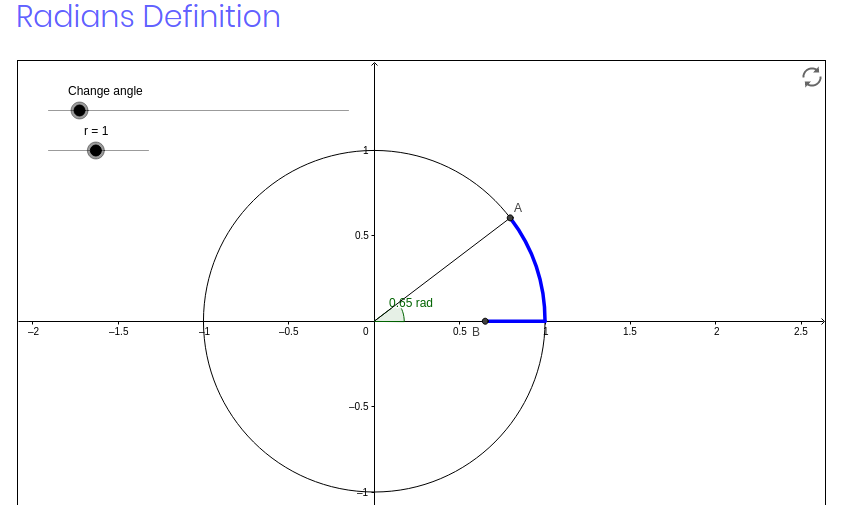
\includegraphics[scale=0.5]{img/Trigon1}
\caption{Definición de radián}
\label{img:radian}
\end{figure}

Utilizando geogebra (ver \ref{img:razones}) las razones trigonométricas en la circunferencia goniométrica. 
\begin{itemize}
	\item ¿De dónde vienen los nombres? 
	\item ¿Triángulos rectángulos para aplicar Pitágoras?
\end{itemize}

\begin{figure}
\centering
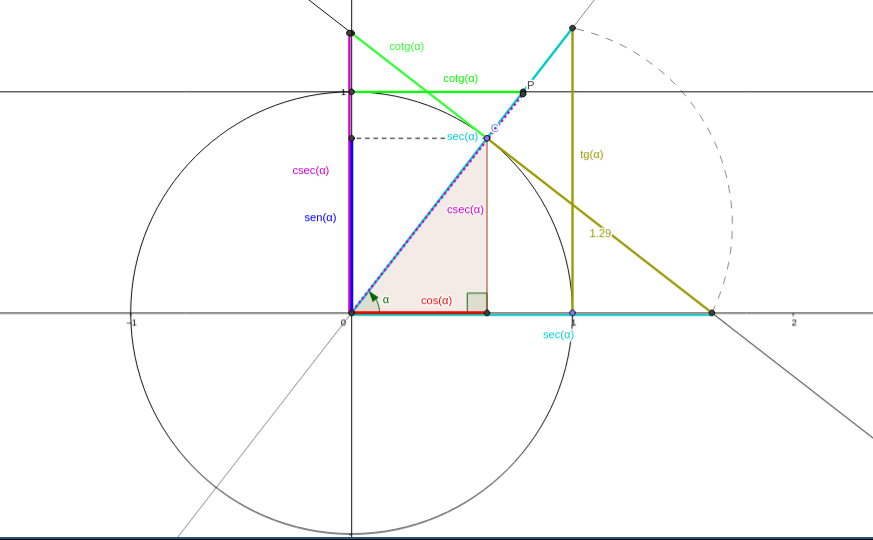
\includegraphics[scale=0.5]{img/Trigon2}
\caption{Razones trigonométricas}
\label{img:razones}
\end{figure}


Proyectando el libro, explicar:
\begin{itemize}
	\item Identidades trigonométricas (página 80). Ojo al "ten en cuenta de la izquierda".
	\item Signo de las razones trigonométricas (página 77).
	\item Reducción al primer cuadrante (página 78).
	\item Tabla de valores notables.
	\item Ángulos complementarios.
\end{itemize}

Ejercicios 16 del libro (utilizando las 2 páginas donde vienen todas las fórmulas) [Corregimos proyectando el libro].

Demuestra (corregimos proyectando el libro). 
\[
	\frac{\cosα-\secα}{\senα-\cosecα} = \tg^3α
\]

Deberes: demuestra algebraicamente $\tg^2α+1=\sec^2α$ y $\cotg^2α+1=\cosec^2α$

\section{Identidades trigonométricas}

\subsection{Suma y diferencia de ángulos}

\begin{figure}[hbtp]
\centering
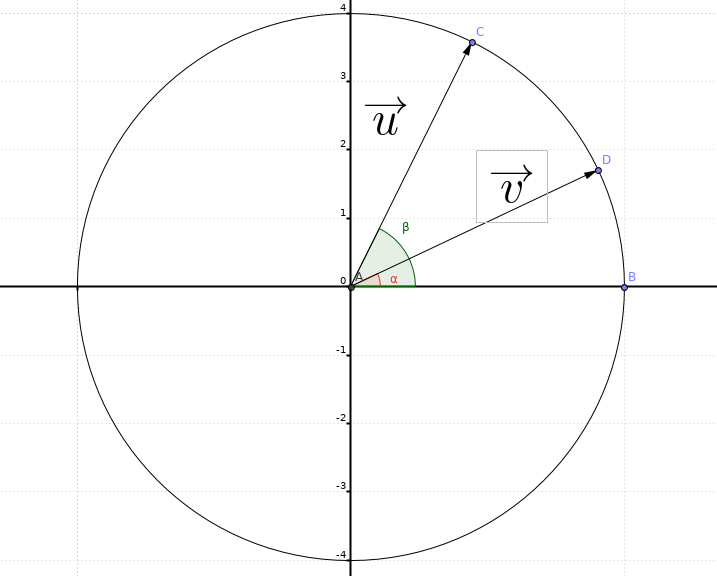
\includegraphics[scale=0.5]{img/Trigon3}
\caption{Razonamiento coseno de la diferencia.}
\label{img:cosenodif}
\end{figure}


Las coordenadas de $\vec{u} = (\cosβ,\senβ)$ y $\vec{v} = (\cosα,\senα)$. Vamos a calcular $\vec{u}·\vec{v}$, teniendo en cuenta que son vectores unitarios.

\[
	\vec{u} · \vec{v} = |\vec{u}| · |\vec{v}| · \cos(β-α) \dimplies (\cosβ,\senβ)·(\cosα,\senα) = \cos(β-α)
\]
\[
	\cos(β-α) = \cosβ\cosα - \senβ\senα
\]
Escribiendo $α=-α$, obtendríamos las razones del ángulo suma.

\begin{example}
	\begin{itemize}
		\item $\sen\left(\rfrac{5π}{12}\right) = \sen\left(\rfrac{2π}{12} + \rfrac{3π}{12}\right)$
	\end{itemize}
\end{example}

Para trabajar (ellos):
\begin{itemize}
		\item $\cos\left(\rfrac{π}{2}+\rfrac{π}{3}\right)$ (ellos)
		\item $\sen\left(\rfrac{π}{12}\right)$ (ellos)
		\item Demuestra: $\displaystyle \tgα+\tgβ = \frac{\sen(α+β)}{\cosα\cosβ}$
\end{itemize}

\paragraph{Multiplicación compleja en forma polar:}

\label{trigon:multicomplejapolar}

$z_1 = r_1\cos(\alpha_1) + r_1·i·\sen(\alpha_1)$ y 
$z_2 = r_2\cos(\alpha_2) + r_2·i·\sen(\alpha_2)$

Haciendo $z_1·z_2 = r_1r_2\left(\cos(\alpha_1)\cos(\alpha_2)-\sen(\alpha_1)\sen(\alpha_2)\right) + i·r_1r_2 \left(
\cos(\alpha_1)\sen(\alpha_2) + \sen(\alpha_1)\cos(\alpha_2)\right) = r_1r_2\left(\cos(\alpha_1+\alpha_2) + i·\sen(\alpha_1+\alpha_2)\right) = {r_1r_2}_{\alpha_1+\alpha_2}
$

\subsubsection{Ángulo doble y ángulo mitad}

\begin{itemize}
	\item $\cos(2α)$ (ellos)
	\item $\sen(2α)$ (ellos)
	\item Calcula $\cos\left(\rfrac{α}{2}\right)$ utilizando $\sen^2β+\cos^2β=1$ y $β=\rfrac{α}{2}$
	\item $\sen\left(\rfrac{β}{2}\right)$
\end{itemize}

Fin clase 2.

\section{Resolución de triángulos}

\subsection{Ecuaciones trigonométricas}

\[\cos(x) = \cos(2x) \overset{?}{\dimplies} x=2x\]

No, ni en un sentido ni en el otro. 

\paragraph{No es $\Rightarrow$} según qué razón trigonométrica y en qué cuerpo estemos trabajando. En $\real\; a = b \implies \cos(a)=\cos(b)$ y $a = b \implies \sen(a)=\sen(b)$ pero 

$a = b \not\implies \tg(a)=\tg(b)$. El ejemplo más claro sería: $x = \rfrac{\pi}{2} \not\implies \tg(x) = \tg(4)$.

\paragraph{No es $\Leftarrow$}


\[
\cos(x) = \cos(2x) \dimplies \cos(x) = \cos^2(x) - \sen^2(x) \dimplies \cos(x) = \cos^2(x) - 1 + \cos^2(x) \dimplies 2\cos^2(x) - \cos(x) -1 = 0
\]

Cambio de variable: $t = \cos(x)$

\[
	2t^2-t-1 = 0 \dimplies \left(t+\rfrac{1}{2}\right)(t-1)=0
\]

Deshacemos el cambio:


\[
\left.
\begin{array}{l}
t_1 = 1\\
t_1 = \cos(x)
\end{array}
\right\} \implies \cos(x) = 1\implies \left\{\begin{array}{l}
x_1 = 0 + 2\pi k\kinz
\end{array}\right.
\]

\[
\left.
\begin{array}{c}
t_2 = \rfrac{-1}{2}\\
t_2 = \cos(x)
\end{array}
\right\} \implies \cos(x) = \rfrac{-1}{2} \implies \left\{\begin{array}{c}
x_2 = \rfrac{2\pi}{3} + 2\pi k\kinz\\
x_3 = \rfrac{-2\pi}{3} + 2\pi k\kinz
\end{array}\right.
\]

Ejercicios 49 y 50.



\subsection{Teorema del seno y del coseno}

\begin{theorem}[Teorema del seno]
En un triágngulo cualquiera se cumplen las siguientes relaciones:

\[\frac{a}{\sen(A)} = \frac{b}{\sen(B)} = \frac{c}{\sen(C)}\]

\end{theorem}

\begin{proof}
Se igualan 2 maneras diferentes de calcular la altura del triángulo.
\end{proof}

\begin{theorem}[Teorema del coseno]
En un triágngulo cualquiera se cumplen las siguientes relaciones:

\begin{itemize}
	\item $a^2 = b^2+c^2 - 2bc\cos(a)$
\end{itemize}

\end{theorem}
\begin{proof}
Se divide el lado $a$ en 2 partes según la altura y se aplica Pitágoras en los 2 triángulos resultantes. 

Se reducen incógnitas hasta que todo dependa sólo de $a,b,c$.
\end{proof}

Problemitas de ejemplo de resolución de triángulos para poder aplicarlo a problemas.

